\documentclass{article}
\usepackage[utf8]{inputenc}

\title{CR_TP2}
\author{philippe.tankmouse }
\date{October 2020}


% New commands declaration

\usepackage[frenchb]{babel}
\usepackage[T1]{fontenc}

\usepackage{natbib,bibentry}
\usepackage{color}
\usepackage{yfonts}
\usepackage{graphicx}
\usepackage{epsfig,subfigure}
\usepackage{amsmath,amssymb,amsfonts}
\usepackage{calc}

\usepackage{array}
\newcolumntype{L}[1]{>{\raggedright\let\newline\\\arraybackslash\hspace{0pt}}m{#1}}
\newcolumntype{C}[1]{>{\centering\let\newline\\\arraybackslash\hspace{0pt}}m{#1}}
\newcolumntype{R}[1]{>{\raggedleft\let\newline\\\arraybackslash\hspace{0pt}}m{#1}}


\DeclareGraphicsExtensions{.eps, .jpg, .png}

\parindent = 0mm

\bibliographystyle{plain}

\hoffset = -20mm
\voffset = -25mm
\textwidth = 160mm
\textheight = 240mm

% \definecolor{lightgray}{gray}{0.2}


\newcommand{\expect}{{\rm I \mkern-2.5mu \nonscript\mkern-.5mu E}}
\newcommand{\equaldef}{\stackrel{d}{=}}
\newcommand{\argmax}{\operatornamewithlimits{argmax}}

\newcommand{\dnu}{16}
\newcommand{\solskip}{10mm}

\renewcommand{\topfraction}{1}
\renewcommand{\bottomfraction}{1}
\renewcommand{\textfraction}{0}

\newcommand{\debutrep}[1]{\color{blue}\begin{center} \hrulefill \textbf{ #1 } \hrulefill \end{center} }
\newcommand{\finrep}{\vspace*{5mm}\hfill $\square$\color{black}\vspace*{5mm}}

\documentclass{article}

\begin{document}

\baselineskip = 4mm
\title{Traitement des Signaux Aléatoires \\
Estimation Spectrale}
\author{\textbf{4 ETI -- CPE Lyon }\\[3mm]
{Travaux Pratiques TSA}}
\date{2020-2021}

\maketitle

\noindent\fbox{
\parbox{\linewidth-2\fboxrule-2\fboxsep}
{ 
\vspace*{2mm}
{\large\bf Noms, Prénoms: }\\[3mm]
{\large\bf Groupe: }\\[3mm]
{\large\bf Date:}\\[2mm]}}
\vspace*{5mm}


\textbf{\Large Objectifs du TP}\\[4mm]

\begin{list}{-}{\setlength{\leftmargin}{3mm} \setlength{\labelwidth}{20mm} \setlength{\labelsep}{2mm} \setlength{\itemsep}{1mm} }
\item Comprendre la notion de densité spectrale d'énergie ou de puissance moyenne
\item Manipuler différents estimateurs empiriques (à partir d'une série temporelle de taille finie) de DSE/DSPM
\item Etudier l'effet du compromis biais-variance d'un estimateur
\end{list}


\vspace*{5mm}

\section{Préparation}

\begin{itemize}
\item[{\bf Question 1}] Comment peut-on calculer simplement la densité spectrale d’énergie (DSE) d’un signal certain d’énergie finie ?

\debutrep{réponse}

\finrep

\item[{\bf Question 2}] Comment est définie la densité spectrale de puissance moyenne (DSPM) d’un processus aléatoire ?

\debutrep{réponse}

\finrep

\item[{\bf Question 3}] Quelles sont les grandeurs qui permettent de chiffrer la qualité d’une estimation dans le cas général ? et la qualité de l’estimation spectrale en particulier.

\debutrep{réponse}

\finrep

\item[{\bf Question 4}] Exprimer la densité spectrale de puissance moyenne (DSPM) GB ( f ) d’un bruit blanc stationnaire centré.

\debutrep{réponse}

\finrep

\item[{\bf Question 5}] Exprimer GX ( f ) , où X(t) est la sortie d’un filtre excité par un bruit blanc centré, en fonction de la DSPM du bruit blanc et des caractéristiques du filtre.

\debutrep{réponse}

\finrep

\item[{\bf Question 6}] En une phrase (sans formule), décrire le procédé de calcul de la DSPM estimée G1 ( f )
d’une séquence aléatoire via l’estimateur simple.

\debutrep{réponse}

\finrep

\item[{\bf Question 7}] Rappeler le mode de graduation d’une TFD-N points en fréquences réduites.

\debutrep{réponse}

\finrep

\item[{\bf Question 8}] Décrire (avec une phrase) le procédé de calcul de la DSPM estimée G2 ( f ) d’une
séquence aléatoire via l’estimateur moyenné.

\debutrep{réponse}

\finrep

\item[{\bf Question 9}] Que signifie le terme «compromis biais-variance» dans le cas de l’estimateur moyenné ?

\debutrep{réponse}

\finrep

\item[{\bf Question 10}] Quelles modifications sont apportées au procédé de calcul de l’estimateur de Welch par rapport à l’estimateur moyenné ?

\debutrep{réponse}

\finrep

\end{itemize}

\clearpage
\setcounter{section}{2}
\section{Estimation de la DSPM d'un bruit blanc gaussien filtré}
\subsection{Génération du bruit à analyser}

A quoi sert l'entier permettant d'initialiser le générateur ?\\

Le problème est qu'il est compliqué d'analyser des processus aléatoire car cela reviendrait à comparer des signaux avec les même caractéristique mais des réalisations différentes. L'option \textit{seed} des fonctions \textit{rnd, rand} sur MATLAB nous permet de fixer la suite de nombre aléatoires dans un ordre précis pour que les n réalisations soit identiques. Ainsi, on étudie un processus pseudo-aléatoire car prédictible.

\subsection{Estimateur spectral simple}
\subsubsection{Script de la fonction {\tt Matlab} développée}

Le code de la focntion \textit{ESS}, il tronqué de sa partie affichage et de ses commentaires pour des raisons de lisibilité mais vous pouvez le retrouver complet en annexes : 
\begin{verbatim}
function  ESS(x,nd,nf,NFFT) ;
    % ---Initialisation des variables ---
    x_seq = x(nd : nf); %Sequence à analyser
    N = nf - nd +1; %Longueur de la sequence
    
    % ---Création de l'estimateur 1 ---
    X = fft(x_seq,NFFT); %Transofrmée N points de la séquence  
    gamma_x_c = ((abs(X)).^2)/N; %Estimation simple
    log_gamma_x_c = 10*log10(gamma_x_c); %Passage au log (forme quadratique donc log * 10)
    
    % ---DSP moyenne vraie et (gamma(f) * Wbm(f))(f)
    [Gth,Gbiais,fth]=sptheo(N,'simple');
    f_abs = 0:1/NFFT:1-1/NFFT;
    
    % ---Partie affichage ---
    figure(2)
    plot(f_abs,log_gamma_x_c,fth,Gth,'k',fth,Gbiais,'r')
    axis([0 0.5 -60 10])
    legend('Estimation de la DSP','DSPMV','Convolution de la DSP et de la fenetre de Barlett')
    title("Etude de l'estimateur simple")
end
\end{verbatim}

\newpage
\subsubsection{Expérimentation}

\begin{enumerate}
\renewcommand{\theenumi}{\Alph{enumi}}
\item Étude du biais et de la variance en fonction du nombre $N$ d'échantillons de bruit

Pour l'étude du biais, nous allons faire varier le paramètre d'entrée N de la fonction \textit{ESS} de 1000 échantillons à 100000 échantillons.

\begin{figure}[h]
\centerline{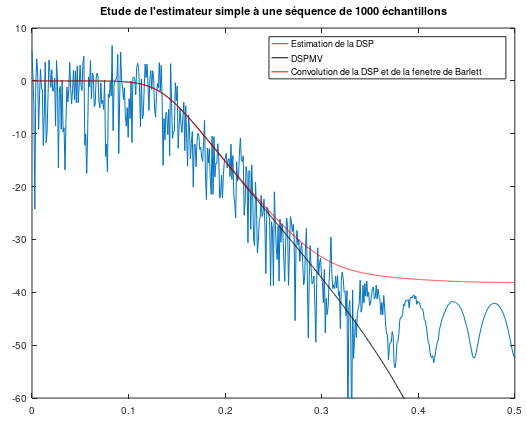
\includegraphics[width=0.52\textwidth]{images/casESN1000.png}}
\caption{$N$ faible (1000)-- indice de début de la séquence à 1}
\end{figure}

\begin{figure}[h]
\centerline{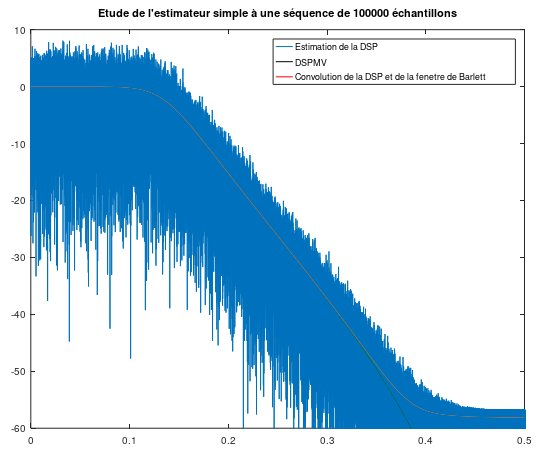
\includegraphics[width=0.52\textwidth]{images/casESN100000.png}}
\caption{$N$ élevé (100 000)-- indice de début de la séquence à 1}
\end{figure}

Sur les figures 1 et 2, nous pouvons observer 3 courbes, la bleu correspond à la densité spectrale obtenues à partir d'une séquence empirique à $N$ points. La courbe noire correspond à la densité spectrale théorique non biaisée et la rouge correspond à la densité spectrale convolué par une fenêtre de BARLETT (donc biaisé). 
Ainsi, nous pouvons constater que si N est faible alors la DS empirique correspond à l'estimateur non-biaisé sur les basses-fréquences mais va être biasié sur les hautes fréquences et une variance qui est "faible" sur toutes la DSP.
Inversement, avec un N important le biais va être "faible" car la courbe bleu suit la DST mais la variance est très importantes. \\
Nous pouvons expliquer ce comportement à l'aide du phénomène de convolution par la fenêtre de BARRET car plus on a une fenêtre tend vers l'inifinie (plus physiquement le signale est long dans le temps) et plus le replie temporelle va être faible donc les hautes fréquences de la DST ne vont pas être impactées par les basses fréquences et le biais diminues. Le problème est que la variance est obtenues à l'aide de la relation :\\
\centerline{$VAR(ES) = \Gamma^2(x) + [1+(sin(2*pi*f*N)/(N*2*pi*f))^2]$}
 
\newline

\item Etude du biais et de la variance en fonction de la réalisation considérée, à $N$ fixé 
\newline
Pour cette étude, nous avons fixé taille du N à 1000 échantillons et l'on obtient les figures suivantes : 

\begin{figure}[h]

\centerline{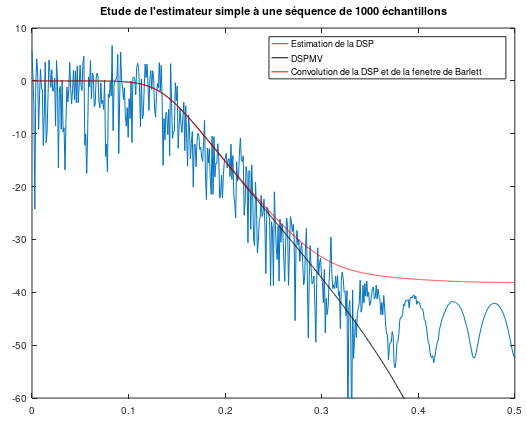
\includegraphics[width=0.55\textwidth]{images/casESN1000.png}}
\caption{$N \sim 1000$ -- indice de début de la séquence à 1}
\end{figure}

\begin{figure}[h]

\centerline{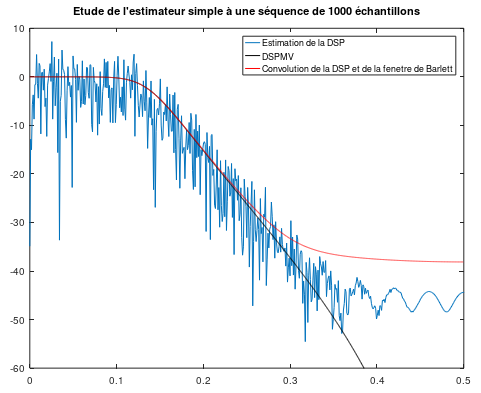
\includegraphics[width=0.55\textwidth]{images/casESN1000PD2000.PNG}}
\caption{$N \sim 1000$  -- indice de début de la séquence fixé à une autre position ($\gg 1000$) dans la séquence}
\end{figure}

Nous pouvons observer que sur les figure 3 et 4 (pour une séquence qui débute à 2000), les courbes obtenues sont semblables. Ce résultat est cohérent car le signal  observé est un bruit blanc Gaussien qui à comme propriété d'être stationnaire donc l'intervalle d'échantillons peut être quelconque car n'influe pas sur l'étude, tant que l'on conserve une même taille $N$. 
\newline

\clearpage
\item Etude du biais et de la variance en fonction du nombre $NFFT$ de FFT
\newline
Pour cette étude, nous avons fixé taille du N à 1000 échantillons et l'on obtient les figures suivantes : 
\begin{figure}[h]
\centerline{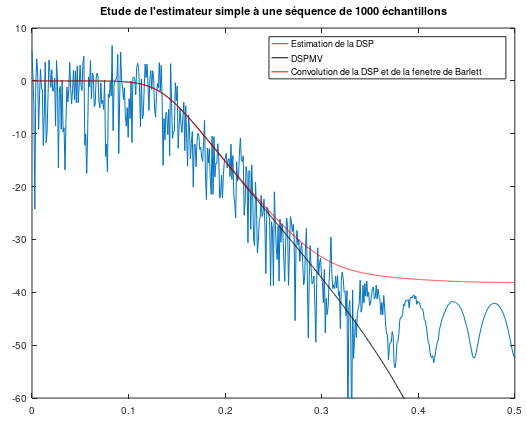
\includegraphics[width=0.55\textwidth]{images/casESN1000.png}}
\caption{$N$ constant -- indice de début de la séquence à 1 -- $NFFT \sim N$}
\end{figure}

\begin{figure}[h]
\centerline{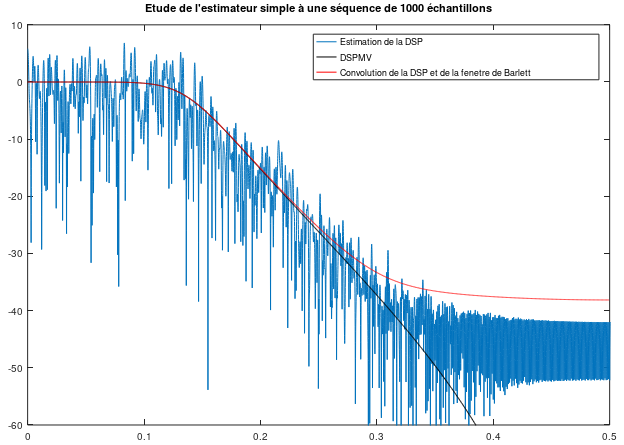
\includegraphics[width=0.55\textwidth]{images/casESN1000FFT214.png}}
\caption{$N$ constant -- indice de début de la séquence à 1 -- $NFFT (2**14) \gg N$}
\end{figure}

Nous pouvons observer que sur les figure 5 et 6 (une FFT sur $2^14$ points), les courbes obtenues sont semblables. Ce résultat est cohérent car pour obtenir les densités spectrales le paramètre $NFFT$ n'influence que le nombre de points pour la Transformé de Fourier à N points. Et va permettre d'augmenter la précisions de la courbe.  Ainsi il ne peut pas influé sur l'étude, tant que l'on prend $NFFT > N$. 
\newline

\item Conclusion
Quel est le principal défaut de l'estimateur simple ?\\
\newline
A l'aide de l'étude réalisé, nous pouvons conclure que l'estimateur simple à comme principale défaut sa variance car N est grand est plus le terme carré pour obtenir la variance va "exploser" et cela devient compliqué d'analyser la courbe. Ainsi cette estimateur n'est pas de bonne qualité.  

\end{enumerate}

\clearpage
\subsection{Estimateur spectral moyenné}

\textbf{On fixera $\mathbf{N=4096}$ dans tout ce qui suit.}

\subsubsection{Script de la fonction {\tt Matlab} développé}

\debutrep{code ci-dessous}
\begin{verbatim}

\end{verbatim}
\finrep


\subsubsection{Expérimentation}

En précisant bien la valeur des paramètres utilisés pour les essais, affichez les figures correspondantes aux conditions indiquées.
\debutrep{figure ci-dessous}

\begin{figure}[h]

\caption{$N=4096$ -- tranches courtes $M = ??? $, $NFFT = ???$}
\end{figure}
\finrep

Commentaires
\debutrep{réponse ci-dessous}

\finrep

\debutrep{figure ci-dessous}
\begin{figure}[h]

\caption{$N=4096$ -- tranches longues $M = ???$, $NFFT = ???$}
\end{figure}

\finrep

Commentaires
\debutrep{réponse ci-dessous}

\finrep

\debutrep{figure ci-dessous}
\begin{figure}[h]

\caption{$N=4096$ -- \og Meilleur \fg compromis biais variance atteint pour $M = ???$, $NFFT = ???$}
\end{figure}

\finrep

Quelle information permettrait d'obtenir le meilleur compromis biais-variance? 

\debutrep{réponse ci-dessous}

\finrep

\clearpage
\section{Estimateur de Welch}

\subsection{Etude préalable des fenêtres}

Quelles différences de comportement fréquentiel peut-on observer pour les 6 fenêtres proposées (lobe principal, lobes latéraux\ldots).

\subsubsection{Script de la fonction {\tt Matlab} développée}

\debutrep{code ci-dessous}
\begin{verbatim}

\end{verbatim}
\finrep

\subsubsection{Expérimentation}

\begin{enumerate}
\renewcommand{\theenumi}{\Alph{enumi}}

\item Etude du biais et de la variance en fonction du taux de recouvrement entre tranches

Pour $N$, $M$ et $NFFT$ fixés et pour une  fenêtre choisie,  tracez les figures correspondantes aux conditions indiquées ci-dessous.

\debutrep{figure ci-dessous}
\begin{figure}[h]

\caption{$N = 4096$ -- $M = ???$, $NFFT = ???$. Choix de fenêtre = ??? -- Recouvrement de $0\%$}
\end{figure}

\begin{figure}[h]

\caption{$N = 4096$ -- $M = ???$, $NFFT = ???$. Choix de fenêtre = ??? -- Recouvrement de $50\%$}
\end{figure}

\finrep

Que permet le recouvrement entre tranches ?

\debutrep{réponse ci-dessous}

\finrep

\item Etude du biais et de la variance en fonction de la fenêtre utilisée

Pour $N$, $M$ et $NFFT$ fixés et pour différents choix de fenêtre,  tracez les figures correspondantes aux conditions indiquées ci-dessous.

\debutrep{figure ci-dessous}
\begin{figure}[h]

\caption{$N = 4096$ -- $M = ???$, $NFFT = ???$. Fenêtre Rectangle -- Recouvrement de $50\%$}
\end{figure}

\begin{figure}[h]

\caption{$N = 4096$ -- $M = ???$, $NFFT = ???$. Fenêtre ??? -- Recouvrement de $50\%$}
\end{figure}

\finrep

Que permet l'utilisation d'une fenêtre autre que rectangulaire ? Expliquer.

\debutrep{réponse ci-dessous}

\finrep

\end{enumerate}

Pour quelles valeurs des paramètres d'analyse obtenez vous le \og meilleur \fg résultat (celui qui vous parait le plus satisfaisant)?

\debutrep{réponse ci-dessous}

Longueur de la séquence analysée $N = ???$ \\
Longueur des tranches $M = ???$ \\
Type de fenêtre ??? \\
Taux de recouvrement = ??? \\
Nombre de points de transformée de Fourier $NFFT = ???$

\finrep

\section{Utilisation des estimateurs précédents pour analyser un signal inconnu}

\subsection{Modification des programmes}

Script d'une des fonctions modifiée

\debutrep{code ci-dessous}
\begin{verbatim}

\end{verbatim}
\finrep

\subsection{Expérimentation}

Afficher les spectres estimés obtenus avec chacune des 3 méthodes étudiées.

\debutrep{figure ci-dessous}
\begin{figure}[h]

\caption{Estimateur spectral simple. \textit{Indiquez tous les paramètres choisis}.}
\end{figure}

\begin{figure}[h]

\caption{Estimateur spectral moyenné. \textit{Indiquez tous les paramètres choisis}.}
\end{figure}

\begin{figure}[h]

\caption{Estimateur spectral de Welch. \textit{Indiquez tous les paramètres choisis}.}
\end{figure}

\finrep

Décrivez précisément la démarche expérimentale suivie. Avec quelle méthode êtes vous capable avec certitude de décrire le contenu fréquentiel de ce signal ?

\debutrep{réponse ci-dessous}

\finrep

\subsubsection{Interprétations}

\begin{enumerate}
\renewcommand{\theenumi}{\Alph{enumi}}

\item Que inconvénient majeur l'utilisation d'une fenêtre (d'apodisation en temps) engendre-t-elle?

\debutrep{réponse ci-dessous}

\finrep

\item Décrire (sans dessin) la forme de la DSPM obtenue.

\debutrep{réponse ci-dessous}

\finrep

\item Quelles informations la forme de cette DSPM apporte-t-elle sur le contenu (la nature) du signal?

\debutrep{réponse ci-dessous}

\finrep

\item Quelles mesures concernant  les caractéristiques du signal peut-on effectuer sur la DSPM?

\debutrep{réponse ci-dessous}

\finrep

\end{enumerate}

\end{document}










































\end{document}
